%%%%%%%%%%%%%%%%%%%%%%%%%%%%%%%%%%%%%%%%%%%%%%%%%%%%%%%%%
%%%  List 对象
%%%%%%%%%%%%%%%%%%%%%%%%%%%%%%%%%%%%%%%%%%%%%%%%%%%%%%%%%

\chapter{Python List 对象}

本章介绍 Python 中 List 对象的实现原理。

\section{List 对象的定义}

cpython 中 List Object 的定义如下。

\begin{lstlisting}[language=C, numbers=left, numbersep=1em, numberstyle=\footnotesize , breaklines=true]
typedef struct {
    PyObject_VAR_HEAD
    PyObject **ob_item;
    Py_ssize_t allocated;
} PyListObject;
\end{lstlisting}

结构非常的简单。其中,ob\_item 保存 List 的元素。例如,执行语句 li = [1, 2, 3],那么 ob\_item 函数指针就会保存 1 2 3 这三个 PyLongObject 的
指针数组,allocated 则保存 List 元素的个数。 

\begin{figure}[htbp]
\centering
  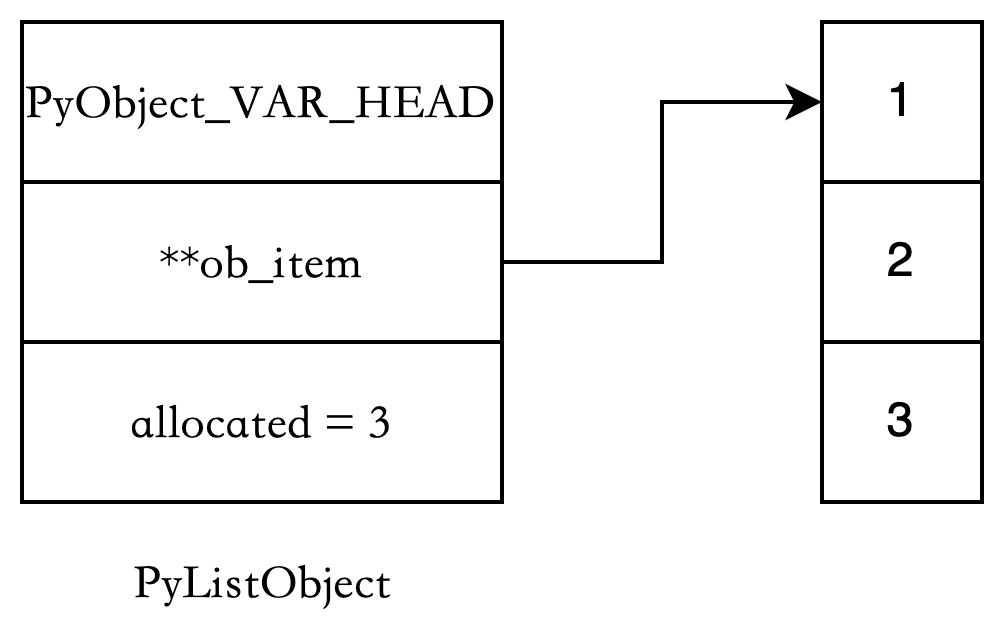
\includegraphics[width=0.5\textwidth]{pictures/ch7_01.png}
  \caption{含有三个元素的 PyListObject \label{fig:scatter}}
\end{figure}

\section{创建 List}

创建 List 是在写 Python 代码时的一个使用频率非常高的操作。一般有两种写法。

\begin{lstlisting}[language=Python, numbers=left, numbersep=1em, numberstyle=\footnotesize , breaklines=true]
a = list()
b = []
\end{lstlisting}

这两种写法最后都会调用 PyList\_New 函数来创建一个  PyListObject 对象。所以看一下 PyList\_New 函数究竟是如何创建一个 List 的。

\begin{lstlisting}[language=C, numbers=left, numbersep=1em, numberstyle=\footnotesize , breaklines=true]
PyObject *
PyList_New(Py_ssize_t size)
{
    // 处理参数错误
    if (size < 0) {
        PyErr_BadInternalCall();
        return NULL;
    }

    struct _Py_list_state *state = get_list_state();
    PyListObject *op;
    // 如果空闲链表中有元素,直接取空闲链表中的元素
    if (state->numfree) {
        state->numfree--;
        op = state->free_list[state->numfree];
        _Py_NewReference((PyObject *)op);
    }
    else {
        // 对 PyList_Type 类型进行 GC,从被释放的元素中获取一个 PyListObject
        op = PyObject_GC_New(PyListObject, &PyList_Type);
        if (op == NULL) {
            return NULL;
        }
    }
    if (size <= 0) {
        op->ob_item = NULL;
    }
    else {
       // 如果参数 size > 0,则申请需要的内存,ob_item 指向申请的内存
        op->ob_item = (PyObject **) PyMem_Calloc(size, sizeof(PyObject *));
        if (op->ob_item == NULL) {
            Py_DECREF(op);
            return PyErr_NoMemory();
        }
    }
    // 设置 ob_size = size
    Py_SET_SIZE(op, size);
    // 设置数组数量
    op->allocated = size;
    _PyObject_GC_TRACK(op);
    return (PyObject *) op;
}
\end{lstlisting}

可以看到,创建一个 List 的过程也是很简洁的,里面提到的 GC 在后面章节会进行详细描述,这里暂且跳过不表。

\section{List 的类型类}

List 的类型类是 PyList\_Type,下面是它的定义。

\begin{lstlisting}[language=C, numbers=left, numbersep=1em, numberstyle=\footnotesize , breaklines=true]
PyTypeObject PyList_Type = {
    PyVarObject_HEAD_INIT(&PyType_Type, 0)
    "list",
    sizeof(PyListObject),
    0,
    (destructor)list_dealloc,                   /* tp_dealloc */
    0,                                          /* tp_vectorcall_offset */
    0,                                          /* tp_getattr */
    0,                                          /* tp_setattr */
    0,                                          /* tp_as_async */
    (reprfunc)list_repr,                        /* tp_repr */
    0,                                          /* tp_as_number */
    &list_as_sequence,                          /* tp_as_sequence */
    &list_as_mapping,                           /* tp_as_mapping */
    PyObject_HashNotImplemented,                /* tp_hash */
    0,                                          /* tp_call */
    0,                                          /* tp_str */
    PyObject_GenericGetAttr,                    /* tp_getattro */
    0,                                          /* tp_setattro */
    0,                                          /* tp_as_buffer */
    Py_TPFLAGS_DEFAULT | Py_TPFLAGS_HAVE_GC |
        Py_TPFLAGS_BASETYPE | Py_TPFLAGS_LIST_SUBCLASS |
        _Py_TPFLAGS_MATCH_SELF | Py_TPFLAGS_SEQUENCE,  /* tp_flags */
    list___init____doc__,                       /* tp_doc */
    (traverseproc)list_traverse,                /* tp_traverse */
    (inquiry)_list_clear,                       /* tp_clear */
    list_richcompare,                           /* tp_richcompare */
    0,                                          /* tp_weaklistoffset */
    list_iter,                                  /* tp_iter */
    0,                                          /* tp_iternext */
    list_methods,                               /* tp_methods */
    0,                                          /* tp_members */
    0,                                          /* tp_getset */
    0,                                          /* tp_base */
    0,                                          /* tp_dict */
    0,                                          /* tp_descr_get */
    0,                                          /* tp_descr_set */
    0,                                          /* tp_dictoffset */
    (initproc)list___init__,                    /* tp_init */
    PyType_GenericAlloc,                        /* tp_alloc */
    PyType_GenericNew,                          /* tp_new */
    PyObject_GC_Del,                            /* tp_free */
    .tp_vectorcall = list_vectorcall,
};
\end{lstlisting}

看起来内容很多,但其实我们并不需要了解这么多。在本章节中,需要关注的元素就如下几个。

\begin{lstlisting}[language=C, numbers=left, numbersep=1em, numberstyle=\footnotesize , breaklines=true]
PyTypeObject PyList_Type = {
    PyVarObject_HEAD_INIT(&PyType_Type, 0)
    "list",
    sizeof(PyListObject),
    0,                                          /* tp_as_number */
    &list_as_sequence,                          /* tp_as_sequence */
    &list_as_mapping,                           /* tp_as_mapping */
    PyObject_HashNotImplemented,                /* tp_hash */
};
\end{lstlisting}

其中 list\_as\_sequence 是 List 作为序列时调用的方法集合,list\_as\_mapping 是 List 作为映射时调用的方法集合,
PyObject\_HashNotImplemented 也值得一看,因为 List 是一个可变的类型,所以在 Python 中,List 是不可以作为
字典的 key 的,如果尝试将 List 作为 key,会爆一个类型错误。

\begin{lstlisting}[language=Python, numbers=left, numbersep=1em, numberstyle=\footnotesize , breaklines=true]
>>> d = {}
>>> d[[233]] = "bilibili"
Traceback (most recent call last):
  File "<stdin>", line 1, in <module>
TypeError: unhashable type: 'list'
\end{lstlisting}

而这个错误恰恰就是 PyObject\_HashNotImplemented 抛出的。

\begin{lstlisting}[language=C, numbers=left, numbersep=1em, numberstyle=\footnotesize , breaklines=true]
Py_hash_t
PyObject_HashNotImplemented(PyObject *v)
{
    PyErr_Format(PyExc_TypeError, "unhashable type: '%.200s'",
                 Py_TYPE(v)->tp_name);
    return -1;
}
\end{lstlisting}

\section{List 部分方法的实现}

要知道 List 中的方法是如何实现的,就需要去了解一下上一节中提到的 list\_as\_sequence 和 list\_as\_mapping 成员。
针对 List 调用的大部分函数都是实现在这两个成员中。List 在 Python 中是同时作为一个序列和一个映射的,所以可以看一下
 List 实现了这两种类型中哪些函数。具体这两个类型每个成员分别表示什么操作可以通过章末列出的资料去了解,这里不一一阐述。

\begin{lstlisting}[language=C, numbers=left, numbersep=1em, numberstyle=\footnotesize , breaklines=true]
static PySequenceMethods list_as_sequence = {
    (lenfunc)list_length,                       /* sq_length */
    (binaryfunc)list_concat,                    /* sq_concat */
    (ssizeargfunc)list_repeat,                  /* sq_repeat */
    (ssizeargfunc)list_item,                    /* sq_item */
    0,                                          /* sq_slice */
    (ssizeobjargproc)list_ass_item,             /* sq_ass_item */
    0,                                          /* sq_ass_slice */
    (objobjproc)list_contains,                  /* sq_contains */
    (binaryfunc)list_inplace_concat,            /* sq_inplace_concat */
    (ssizeargfunc)list_inplace_repeat,          /* sq_inplace_repeat */
};

static PyMappingMethods list_as_mapping = {
    (lenfunc)list_length,
    (binaryfunc)list_subscript,
    (objobjargproc)list_ass_subscript
};
\end{lstlisting}

\subsection{List 的长度}

获取 List 的长度的常用方法是 len() 函数,底层调用的是 list\_length 函数,直接返回 ob\_size 成员。
\begin{lstlisting}[language=C, numbers=left, numbersep=1em, numberstyle=\footnotesize , breaklines=true]
static Py_ssize_t
list_length(PyListObject *a)
{
    return Py_SIZE(a);
}
\end{lstlisting}

\subsection{获取 List 某个位置的元素}

获取 List 某个位置的元素的函数用法一般是下面这样子。

\begin{lstlisting}[language=Python, numbers=left, numbersep=1em, numberstyle=\footnotesize , breaklines=true]
a = [3, 2, 1]
a[1]  # 2
a[0:2] # [0, 1]
\end{lstlisting}

其中 a[1] 就是获取 List a 的 第2 个位置的元素(元素位置从 0 开始计数)。底层函数是 list\_item。

\begin{lstlisting}[language=C, numbers=left, numbersep=1em, numberstyle=\footnotesize , breaklines=true]
static PyObject *
list_item(PyListObject *a, Py_ssize_t i)
{
    if (!valid_index(i, Py_SIZE(a))) {
        if (indexerr == NULL) {
            indexerr = PyUnicode_FromString(
                "list index out of range");
            if (indexerr == NULL)
                return NULL;
        }
        PyErr_SetObject(PyExc_IndexError, indexerr);
        return NULL;
    }
    Py_INCREF(a->ob_item[i]);
    return a->ob_item[i];
}
\end{lstlisting}

a[0:2] 是获取 List 中某个区间的元素,底层调用的是 List 作为映射类型的一个方法 list\_subscript。
\begin{lstlisting}[language=C, numbers=left, numbersep=1em, numberstyle=\footnotesize , breaklines=true]
static PyObject *
list_subscript(PyListObject* self, PyObject* item)
{
    if (_PyIndex_Check(item)) {
        Py_ssize_t i;
        i = PyNumber_AsSsize_t(item, PyExc_IndexError);
        if (i == -1 && PyErr_Occurred())
            return NULL;
        if (i < 0)
            i += PyList_GET_SIZE(self);
        return list_item(self, i);
    }
    // 如果是取数组的范围,那么 item 的类型是 slice
    else if (PySlice_Check(item)) {
        Py_ssize_t start, stop, step, slicelength, i;
        size_t cur;
        PyObject* result;
        PyObject* it;
        PyObject **src, **dest;
        // 取出开始 结尾和步长
        if (PySlice_Unpack(item, &start, &stop, &step) < 0) {
            return NULL;
        }
        // 求需要返回的元素个数,可以简单理解为 (stop - start - 1) / step + 1
        slicelength = PySlice_AdjustIndices(Py_SIZE(self), &start, &stop,
                                            step);
        // start = stop, step = 1 的情况
        if (slicelength <= 0) {
            return PyList_New(0);
        }
        // 如果 step = 1,直接返回 List[start, stop)
        else if (step == 1) {
            return list_slice(self, start, stop);
        }
        else {
            // 如果 step > 1,那么闲创建一个 List, 再将对应位置的元素插入到创建的 List
            result = list_new_prealloc(slicelength);
            if (!result) return NULL;

            src = self->ob_item;
            dest = ((PyListObject *)result)->ob_item;
            for (cur = start, i = 0; i < slicelength;
                 cur += (size_t)step, i++) {
                it = src[cur];
                Py_INCREF(it);
                dest[i] = it;
            }
            Py_SET_SIZE(result, slicelength);
            return result;
        }
    }
    else {
        PyErr_Format(PyExc_TypeError,
                     "list indices must be integers or slices, not %.200s",
                     Py_TYPE(item)->tp_name);
        return NULL;
    }
}
\end{lstlisting}

\subsection{设置 List 的元素}

设置 List 的元素和获取 List 的元素一样,也分为两种情况,分别是一次设置一个位置上的元素
和一次设置多个位置上的元素。和获取元素不同的是,这两种情况的入口函数只有一个,都是
映射类型的方法 list\_ass\_subscript。

\begin{lstlisting}[language=Python, numbers=left, numbersep=1em, numberstyle=\footnotesize , breaklines=true]
a = [3, 2, 1]
a[1] = 100
a[0:2] = []
\end{lstlisting}

\begin{lstlisting}[language=C, numbers=left, numbersep=1em, numberstyle=\footnotesize , breaklines=true]
static int
list_ass_subscript(PyListObject* self, PyObject* item, PyObject* value)
{
    // 如果是 a[1] = 100 这种语法,则进入下面这个分支
    if (_PyIndex_Check(item)) {
        Py_ssize_t i = PyNumber_AsSsize_t(item, PyExc_IndexError);
        if (i == -1 && PyErr_Occurred())
            return -1;
        if (i < 0)
            i += PyList_GET_SIZE(self);
        // 调用序列类型的方法设置位置 i 的值为 value
        return list_ass_item(self, i, value);
    }
    // 如果是 a[0:2] = [] 这种语法,则进入下面这个分支
    else if (PySlice_Check(item)) {
        Py_ssize_t start, stop, step, slicelength;

        if (PySlice_Unpack(item, &start, &stop, &step) < 0) {
            return -1;
        }
        slicelength = PySlice_AdjustIndices(Py_SIZE(self), &start, &stop,
                                            step);
        // 如果是 a[0:2] = [], 这种形式,把 a[0:2] 替换为 []
        if (step == 1)
            return list_ass_slice(self, start, stop, value);
        // 处理 s[5:2] = [..] 这种开始位置大于结束位置的情况
        // 将结束位置改为开始位置,相当于在开始位置之后插入
        if ((step < 0 && start < stop) ||
            (step > 0 && start > stop))
            stop = start;
        // 这种情况下直接删除选中的 List 区域,但是不知道怎么构造这个例子
        if (value == NULL) {
            /* delete slice */
            PyObject **garbage;
            size_t cur;
            Py_ssize_t i;
            int res;

            if (slicelength <= 0)
                return 0;

            if (step < 0) {
                stop = start + 1;
                start = stop + step*(slicelength - 1) - 1;
                step = -step;
            }

            garbage = (PyObject**)
                PyMem_Malloc(slicelength*sizeof(PyObject*));
            if (!garbage) {
                PyErr_NoMemory();
                return -1;
            }
            for (cur = start, i = 0;
                 cur < (size_t)stop;
                 cur += step, i++) {
                Py_ssize_t lim = step - 1;

                garbage[i] = PyList_GET_ITEM(self, cur);

                if (cur + step >= (size_t)Py_SIZE(self)) {
                    lim = Py_SIZE(self) - cur - 1;
                }

                memmove(self->ob_item + cur - i,
                    self->ob_item + cur + 1,
                    lim * sizeof(PyObject *));
            }
            cur = start + (size_t)slicelength * step;
            if (cur < (size_t)Py_SIZE(self)) {
                memmove(self->ob_item + cur - slicelength,
                    self->ob_item + cur,
                    (Py_SIZE(self) - cur) *
                     sizeof(PyObject *));
            }

            Py_SET_SIZE(self, Py_SIZE(self) - slicelength);
            res = list_resize(self, Py_SIZE(self));

            for (i = 0; i < slicelength; i++) {
                Py_DECREF(garbage[i]);
            }
            PyMem_Free(garbage);

            return res;
        }
        else {
            // 处理 a[0:20:2] = [..] 这种情况
            PyObject *ins, *seq;
            PyObject **garbage, **seqitems, **selfitems;
            Py_ssize_t i;
            size_t cur;

            /* protect against a[::-1] = a */
            if (self == (PyListObject*)value) {
                seq = list_slice((PyListObject*)value, 0,
                                   PyList_GET_SIZE(value));
            }
            else {
                seq = PySequence_Fast(value,
                                      "must assign iterable "
                                      "to extended slice");
            }
            if (!seq)
                return -1;

            if (PySequence_Fast_GET_SIZE(seq) != slicelength) {
                PyErr_Format(PyExc_ValueError,
                    "attempt to assign sequence of "
                    "size %zd to extended slice of "
                    "size %zd",
                         PySequence_Fast_GET_SIZE(seq),
                         slicelength);
                Py_DECREF(seq);
                return -1;
            }

            if (!slicelength) {
                Py_DECREF(seq);
                return 0;
            }

            garbage = (PyObject**)
                PyMem_Malloc(slicelength*sizeof(PyObject*));
            if (!garbage) {
                Py_DECREF(seq);
                PyErr_NoMemory();
                return -1;
            }

            selfitems = self->ob_item;
            seqitems = PySequence_Fast_ITEMS(seq);
            for (cur = start, i = 0; i < slicelength;
                 cur += (size_t)step, i++) {
                garbage[i] = selfitems[cur];
                ins = seqitems[i];
                Py_INCREF(ins);
                selfitems[cur] = ins;
            }

            for (i = 0; i < slicelength; i++) {
                Py_DECREF(garbage[i]);
            }

            PyMem_Free(garbage);
            Py_DECREF(seq);

            return 0;
        }
    }
    else {
        PyErr_Format(PyExc_TypeError,
                     "list indices must be integers or slices, not %.200s",
                     Py_TYPE(item)->tp_name);
        return -1;
    }
}
\end{lstlisting}

设置 List 元素的函数还是比较复杂的,不过以不同的参数分为了几类主要的情况,都在上面进行了介绍。

\section{List 添加元素}

List 可以使用 append 和 extend 方法来添加元素,接下来就分析下这两个方法的细节。

\begin{lstlisting}[language=Python, numbers=left, numbersep=1em, numberstyle=\footnotesize , breaklines=true]
>>> a = []
>>> a.append([1,2,3])
>>> a
[[1, 2, 3]]
>>> a.extend([4,5,6])
>>> a
[[1, 2, 3], 4, 5, 6]
\end{lstlisting}

append 方法会在原来的 List 对象后面添加一个新元素,不过每次只能添加一个。
extend 方法则是将新的元素“解包”之后再添加到原来的 List 的最后面。

append 方法的实现相对来说比较简单,毕竟每次只需要考虑添加一个元素。所以代码
也比较简洁,主要分为两步。第一步检查是否需要扩容,如果需要的话,进行扩容。
第二步是将 append 的参数(一个 PyObject)添加到原本的 List 数组的末尾。
\begin{lstlisting}[language=C, numbers=left, numbersep=1em, numberstyle=\footnotesize , breaklines=true]
static PyObject *
list_append(PyListObject *self, PyObject *object)
{
    if (app1(self, object) == 0)
        Py_RETURN_NONE;
    return NULL;
}

static int
app1(PyListObject *self, PyObject *v)
{
    Py_ssize_t n = PyList_GET_SIZE(self);

    assert (v != NULL);
    assert((size_t)n + 1 < PY_SSIZE_T_MAX);
    // 数组扩容,不一定会发生在次分配
    if (list_resize(self, n+1) < 0)
        return -1;

    Py_INCREF(v);
    // 将新的 PyObject 添加到数组的最后面
    PyList_SET_ITEM(self, n, v);
    return 0;
}
\end{lstlisting}

extend 方法相比于 append 方法要复杂一些。主要是因为 extend 方法的参数可能性比较多,list、tuple,
和一些可迭代的对象类似于 set 等都可以作为 extend 方法的参数。大体情况分两种,第一种是 如果参数
是 list、tuple 对象或者 list 自身,那么先扩容,再将参数的所有成员添加到本 list 对象的数组中。第二种
情况是如果参数是一个可迭代对象,那么先获取可迭代对象的数量,对本 list 进行扩容,接着遍历一次可
迭代对象,将所有成员添加到本 list 的数组中。

\begin{lstlisting}[language=C, numbers=left, numbersep=1em, numberstyle=\footnotesize , breaklines=true]
static PyObject *
list_extend(PyListObject *self, PyObject *iterable)
{
    PyObject *it;      /* iter(v) */
    Py_ssize_t m;                  /* size of self */
    Py_ssize_t n;                  /* guess for size of iterable */
    Py_ssize_t mn;                 /* m + n */
    Py_ssize_t i;
    PyObject *(*iternext)(PyObject *);
    // 如果 iterable 参数是 List, Tuple 类型,或者是 List 自身(那么当然也是一个 List 了,所以为什么还
    // 要检查self == iterable),就进入下面这个分支
    if (PyList_CheckExact(iterable) || PyTuple_CheckExact(iterable) ||
                (PyObject *)self == iterable) {
        PyObject **src, **dest;
        // 如果 iterable 是一个 List 或者 Tuple 的话,iterable 还是自身
        // 如果是一个可迭代对象的话,
        iterable = PySequence_Fast(iterable, "argument must be iterable");
        if (!iterable)
            return NULL;
        n = PySequence_Fast_GET_SIZE(iterable);
        if (n == 0) {
            /* short circuit when iterable is empty */
            Py_DECREF(iterable);
            Py_RETURN_NONE;
        }
        m = Py_SIZE(self);
        assert(m < PY_SSIZE_T_MAX - n);
        // 数组扩容
        if (list_resize(self, m + n) < 0) {
            Py_DECREF(iterable);
            return NULL;
        }
        src = PySequence_Fast_ITEMS(iterable);
        dest = self->ob_item + m;
        // 将 iterable 内的元素全部添加到 List 的数组之后
        for (i = 0; i < n; i++) {
            PyObject *o = src[i];
            Py_INCREF(o);
            dest[i] = o;
        }
        Py_DECREF(iterable);
        Py_RETURN_NONE;
    }
    // iterable 是一个类似 set 的可迭代对象,则进入下面的分支
    it = PyObject_GetIter(iterable);
    if (it == NULL)
        return NULL;
    iternext = *Py_TYPE(it)->tp_iternext;

    // 获取 iterable 中元素数量
    n = PyObject_LengthHint(iterable, 8);
    if (n < 0) {
        Py_DECREF(it);
        return NULL;
    }
    m = Py_SIZE(self);
    if (m > PY_SSIZE_T_MAX - n) {
         // 如果进入了这个分支,那么要不然是 n 的值错误了,不用管
         // 要不然最后肯定会在下面的循环中导致系统内存消耗完,救不了
    }
    else {
        mn = m + n;
        // 扩容
        if (list_resize(self, mn) < 0)
            goto error;
        Py_SET_SIZE(self, m);
    }

    // 将 iterable 内的元素全部添加到 List 的数组之后
    for (;;) {
        PyObject *item = iternext(it);
        if (item == NULL) {
            if (PyErr_Occurred()) {
                if (PyErr_ExceptionMatches(PyExc_StopIteration))
                    PyErr_Clear();
                else
                    goto error;
            }
            break;
        }
        if (Py_SIZE(self) < self->allocated) {
            /* steals ref */
            PyList_SET_ITEM(self, Py_SIZE(self), item);
            Py_SET_SIZE(self, Py_SIZE(self) + 1);
        }
        else {
            int status = app1(self, item);
            Py_DECREF(item);  /* append creates a new ref */
            if (status < 0)
                goto error;
        }
    }

    // 一个小优化,如果上面扩容阔的太大了,这里再进行缩容,不过感觉是多此一举
    if (Py_SIZE(self) < self->allocated) {
        if (list_resize(self, Py_SIZE(self)) < 0)
            goto error;
    }

    Py_DECREF(it);
    Py_RETURN_NONE;

  error:
    Py_DECREF(it);
    return NULL;
}
\end{lstlisting}

\section{List 排序}



\section{参考}

\begin{itemize}
\item \href{https://docs.python.org/3/c-api/typeobj.html}{Type Objects}
\end{itemize}



